%--------------------
% Packages
% -------------------
\documentclass[11pt,a4paper]{article}
\usepackage[utf8]{inputenc}
\usepackage[T1]{fontenc}
%\usepackage{gentium}
\usepackage{xcolor}
\usepackage{graphicx}
\usepackage{subcaption}
\usepackage{titlesec}
\usepackage[pdftex]{graphicx} % Required for including pictures
\usepackage[english]{babel} 
\usepackage[pdftex,linkcolor=black,pdfborder={0 0 0}]{hyperref} % Format links for pdf
\usepackage{calc} % To reset the counter in the document after title page
\usepackage{enumitem} % Includes lists
\usepackage{parskip}
\usepackage{float}

\frenchspacing % No double spacing between sentences
\linespread{1} % Set linespace
\usepackage[a4paper, lmargin=0.1\paperwidth, rmargin=0.1\paperwidth, tmargin=0.1\paperheight, bmargin=0.1\paperheight]{geometry} %margins
%\usepackage{parskip}

\usepackage[all]{nowidow} % Tries to remove widows
\usepackage[protrusion=true,expansion=true]{microtype} % Improves typography, load after fontpackage is selected

\usepackage[backend=biber, style=numeric]{biblatex}
\usepackage{csquotes}
\addbibresource{sample.bib} 

%-----------------------
% Set pdf information and add title, fill in the fields
%-----------------------
\hypersetup{ 	
pdfsubject = {},
pdftitle = {},
pdfauthor = {}
}
%-----------------------
% Begin document
%-----------------------
\begin{document}
\title{\vspace{-2.0cm}COMS4762 ML4FG: Autoencoders are all single-cell data integration  needs}
\author{Vinayak Kannan (vk2364), Ishaq Kothari (ink2109), Erica Koyama (ek3371)}
\date{}
\maketitle
\section*{Abstract}
We present a novel method for integrating single cell modalities by handling missing features. We improve on the preexisting StabMap framework by replacing PCA dimensional reduction steps with three distinct auto-encoder frameworks. We find that auto-encoders frameworks utilizing transformer layers to handle missingness effectively handle missingness comparing our results with StabMap embeddings. We found that a Multi-Modal Early Fusion Transformer VAE Model handled missing features the best while clearly seperating each of the cell modalities.
\section{Introduction}
Single-cell multiomics sequencing technologies enable simultaneous measurement of cellular characteristics, such as RNA expression and protein abundance. This comprehensive data allows for more detailed cell characterization and facilitates the exploration of relationships between distinct omics layers. However, datasets often consist of non-overlapping modalities, leading to a mosaic-like structure where integration across these modalities becomes challenging. Existing mosaic integration methods typically rely on overlapping features between modalities, which can result in the loss of valuable information from non-overlapping areas.

StabMap addresses this challenge by incorporating both overlapping and non-overlapping features to provide an accurate cell characterization without losing critical data \cite{stabmap}. Building on the StabMap framework, we focus on mitigating data loss in mosaic integration to improve cell characterization and uncover deeper insights into cross-modality relationships. Specifically, we propose three distinct Variational Autoencoder (VAE)-based pipelines that operate within the combined feature space of the dataset, generating a lower-dimensional embedding representation of the single-cell data. This approach replaces the principal component analysis (PCA) embedding step used in StabMap. To ensure comparability, we evaluate our method using the same datasets employed in the original StabMap study.

\section{Methods}
\subsection{Data Preprocessing}
Data were sourced from the \textit{pbmc-10x} dataset, which includes both RNA expression and Assay for Transposase-Accessible Chromatin (ATAC) data. The RNA gene expression data were preprocessed using log-normalization, and highly variable genes were identified with the \texttt{Seurat V3} package. For the ATAC-seq data, we applied the Term Frequency-Inverse Document Frequency (TF-IDF) method to assign weights to open chromatin regions, emphasizing those of higher importance within the dataset.

To prepare for deep learning with PyTorch, we developed a custom class to streamline data processing and facilitate integration with autoencoders. This class takes as inputs the preprocessed \texttt{atac\_data}, \texttt{multimodal\_data}, and annotated cell types. We calculated the number of unique cell types in the dataset and organized the data into three subsets: one containing features unique to RNA expression, one containing features unique to ATAC-seq, and one containing shared features between the RNA and ATAC-seq modalities.

We also implemented a collate function to convert the RNA and ATAC data into tensors, ensuring efficient processing within PyTorch. Attention masks were employed to highlight regions of open chromatin and genes with non-zero accessibility scores.

Our approach for training the autoencoder model involved using RNA data for training, while embeddings were tested on the chromatin data. To assess cell similarity in the embedding space, we used a soft KNN metric, enabling backpropagation during model training.

Initial analysis of the cell types in the dataset revealed that 32\% of the data corresponded to Myeloid Cells, while 68\% were Lymphoid Cells. Regarding features, the training dataset contained a total of 1,740 features, with 952 features shared between the multiome and ATAC-seq data, and 788 features unique to the ATAC-seq dataset. Notably, no features were unique to the multiome dataset.

The challenge in our data integration lies in separating the dataset into distinct modalities. Fully resolved embeddings would ideally capture the unique characteristics of each modality while accurately representing their relationships, ensuring that shared and modality-specific features are properly disentangled.



%(Information about our data)
%# of cell
%# of features


\subsection{VAE Implementation}
In all our approaches, we replaced StabMap using different implementations of VAEs. We used the same single-cell data matrix as in the original study. Performance was evaluated by comparing the results against those reported in the paper.

\subsubsection{Multi-Modal Early Fusion Transformer VAE }
Early fusion multi-modal models are designed to integrate information from multiple modalities as the input of a deep learning architecture. This approach combines raw data from different sources before any significant processing occurs, allowing the model to learn joint representations. In early fusion, the diverse input modalities are concatenated into a unified input vector. In addition, a modality embedding is learned / trained to help the model distinguish between modalities. This method enables the model to leverage the complementary information from various modalities early in the pipeline, leading to more comprehensive and nuanced representations of the combined tensor in the final hidden state. Early fusion can be particularly effective when there are strong correlations between the different modalities, as it allows the model to learn these relationships from the outset \cite{earlyfusion}.

Three iterations of the multi-modal model were tested. Given that the output of StabMap is cross-modality embeddings, this method was trained to output embeddings. These embeddings are visualized in the Results section.

This model tested projecting each RNA / Chromatin expression value by performing the following steps. Firstly, the input is batch normalized to handle large values; this also has the effect of making zero values provided as input non-zero. This effect is useful as, in the next step, the input vector is multiplied (element-by-element wise) by the boolean mask for missing values that is created during pre-processing. This means that  the missing values are zeroed out while zero values provided as input are still preserved as non-zero entities for the model to use later. Afterward, the input is expanded into a higher-dimensional space as specified by the provided hyperparameter via a linear layer (note that the linear projection does not include bias so that missing values (which have zero values) do not have any input into the projection). Finally, the tensor is concatenated across modalities and passed into the transformer architecture. Cross Entropy was used as the loss function

The model architecture described above is visualized below:

\begin{figure}[H]
    \centering
    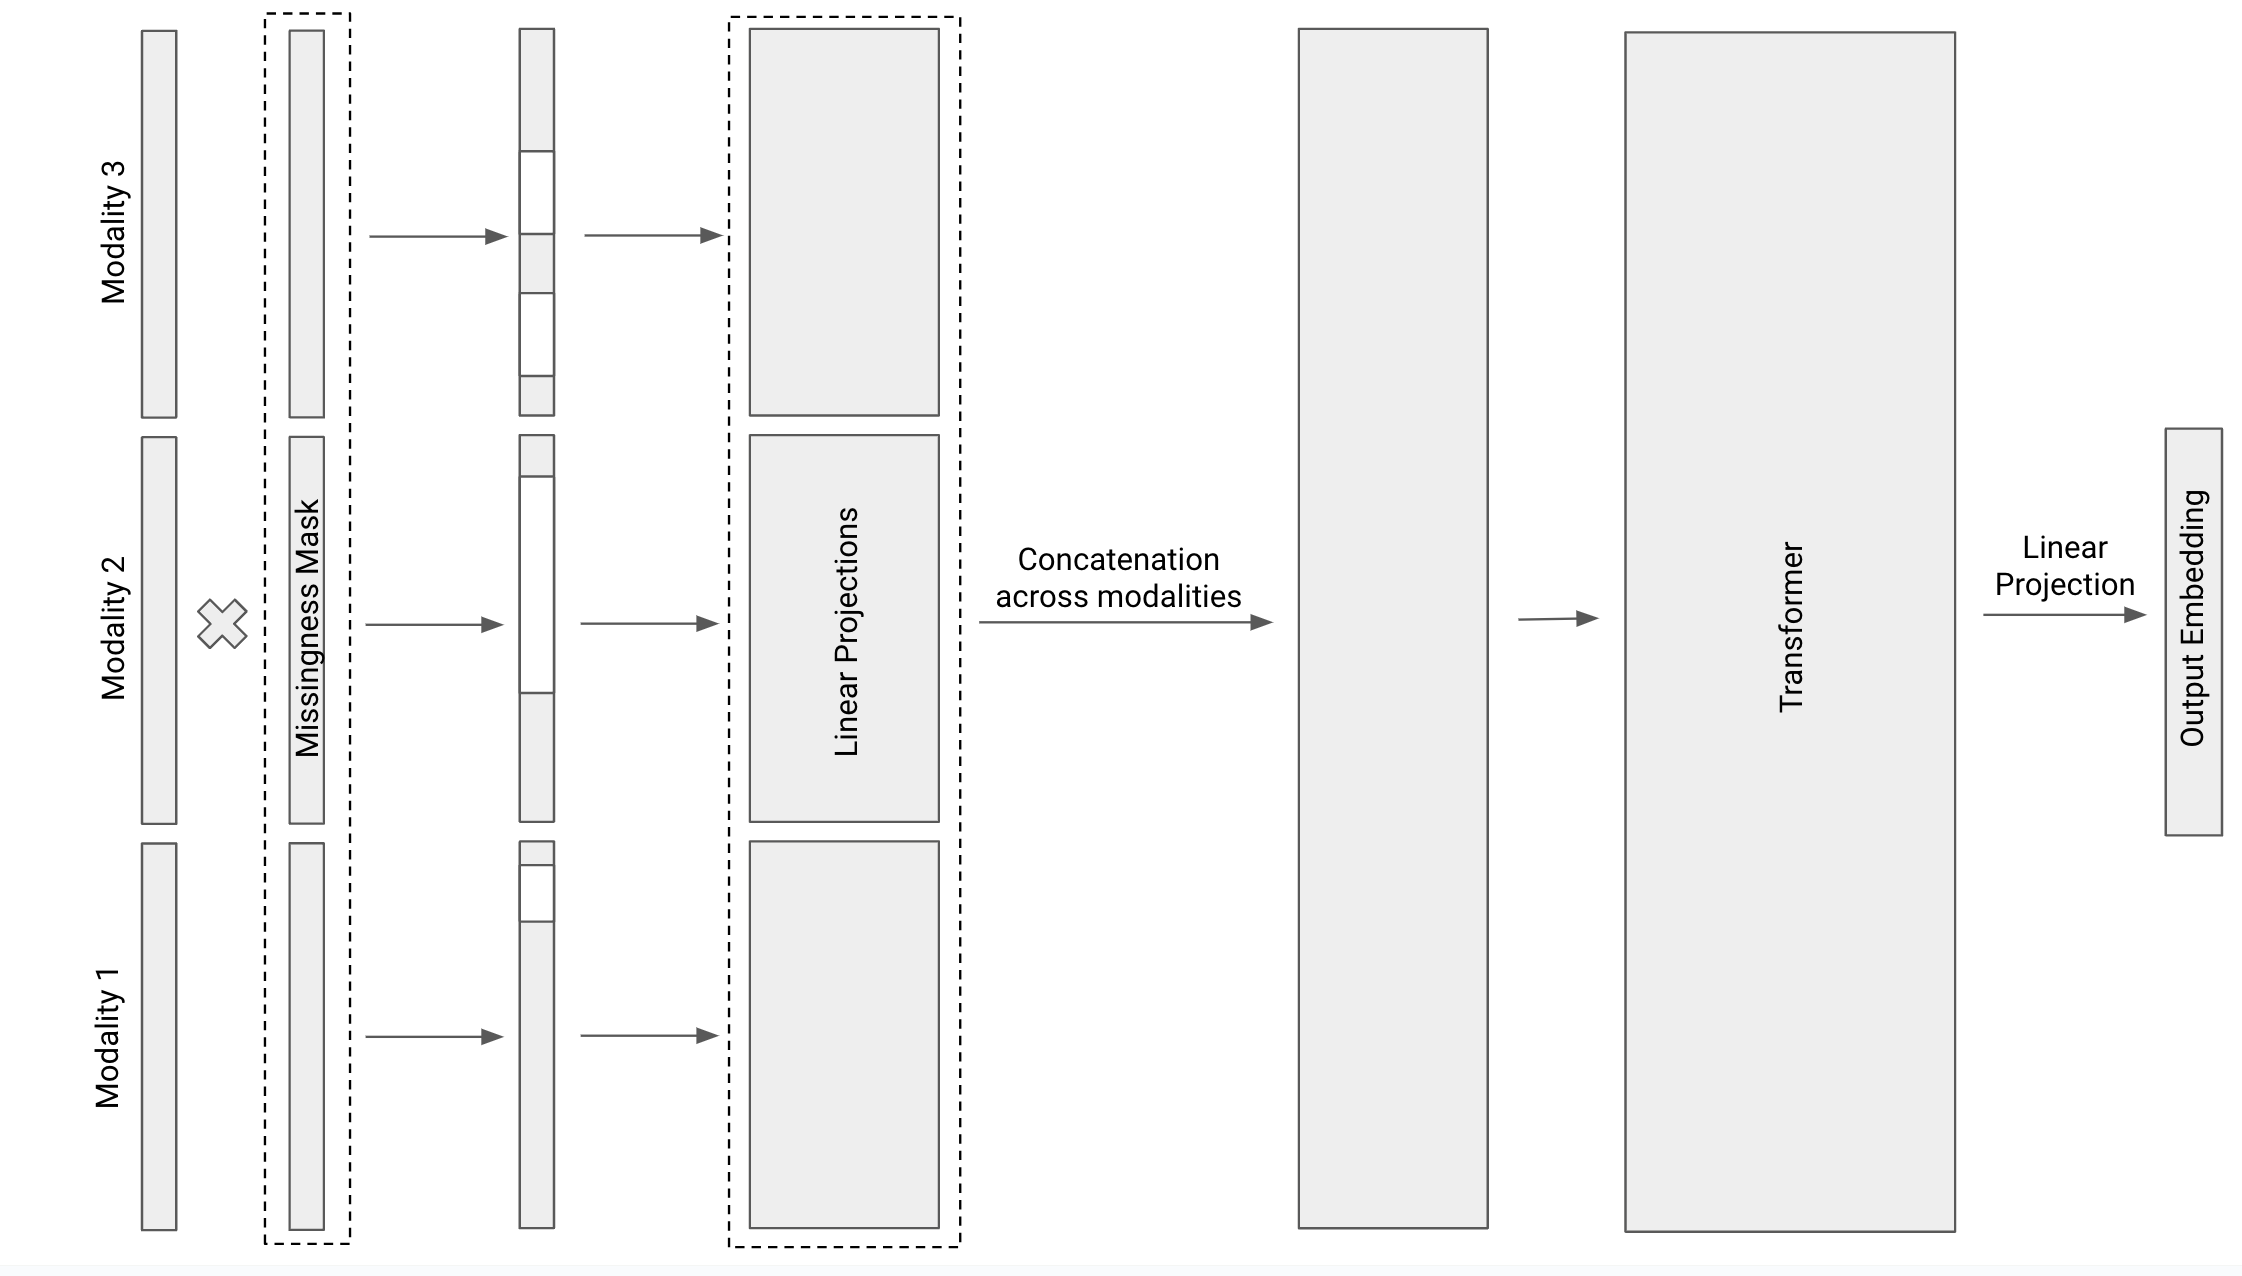
\includegraphics[width=0.5\linewidth]{Figure 2 Final.png}
    \caption{MM Early Fusion Transformer VAE}
    \label{fig:enter-label}
\end{figure}

\subsubsection{Hyperbolic Multi-Modal Early Fusion Transformer VAE }
Hyperbolic space's constant negative curvature allows it to have exponentially growing neighborhood sizes. This property provides an advantage over Euclidean spaces when representing data with latent hierarchical structures, where entities have tree-like relationships \cite{chami2020treescontinuousembeddingsback}. Although we are unsure if the data has latent hierarchy, we chose to explore the hyperbolic model to test its potential for capturing such structures.

The hyperbolic model enhances the Multi-Modal Early Fusion Transformer VAE by mapping the transformer encoder's output embeddings into a curvature -1 hyperbolic latent space. Specifically, the mean plane and log-variance of the latent variables is computed, then the latent mean vector is transformed to a point on the hyperbolic manifold by using the exponential map. 

This transformation enables the model to better capture, if present, the latent relationships across multiple modalities. By using the reparametrization trick and manifold operations, the model projects the latent variables into hyperbolic space.

\subsubsection{MLP-based VAE}
VAEs function by encoding an input matrix to a latent space and then decoding it, while adding a Gaussian constraint so that the encoder returns a mean and standard deviation vector for our learned representation. The MLP-VAE architecture is simple to implement in PyTorch, consisting of a fully connected neural network for both the encoder and decoder. Furthermore, an MLP-based VAE can be flexibly applied to different datasets without changes to the underlying architecture. This is a helpful consideration when applying our embedding to datasets with different modalities. We handled missingness in our MLP-VAE by appylying the same batch normalization strategy and masking strategy as applied to our Multi-Modal Early Fusion Transformer VAE.

\begin{figure}[H]
    \centering
    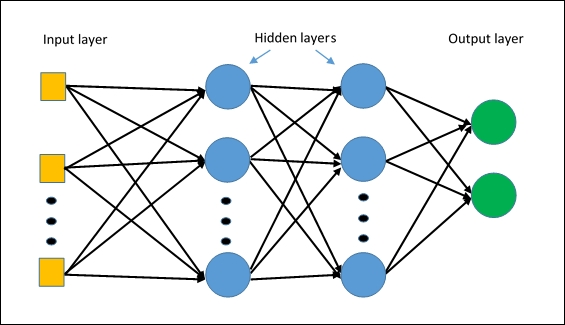
\includegraphics[width=0.5\linewidth]{mlp.png}
    \caption{Architecture for MLP based VAE}
    \label{fig:enter-label}
\end{figure}


\section{Results}

All metrics below are reported on the test dataset. Our code can be found here: https://github.com/Vinayak-Kannan/ML4FG-StabMap-Project
\begin{center}
\begin{tabular}{||c c c||} 
 \hline
 Method & KNN Accuracy (K = 5) & Jaccard Similarity Mean  \\ [0.5ex] 
 \hline\hline
 StabMap Seurat (baseline) & 0.59 & 0.03 \\ 
 \hline
 Multi-Modal Early Fusion Transformer VAE & 0.99 & 0.98 \\
 \hline
 MLP VAE & 0.78 & 0.98 \\
 \hline
 Hyperbolic Multi-Modal Early Fusion Transf. VAE & 0.68 & 0.99 \\
 \hline
\end{tabular}
\end{center}

\subsection{MLP-based VAE}
The following hyperparameters were used in this model:
 \begin{itemize}
     \item Linear Projection Dimension: 6
     \item Number of Hidden Layers: 4
     \item Latent Dimension = 32
     \item Output Embedding Size: 2
     \item Number of Parameters in Model: 37,593
 \end{itemize}

The train and test loss are shown below:

\begin{figure}[H]
    \centering
    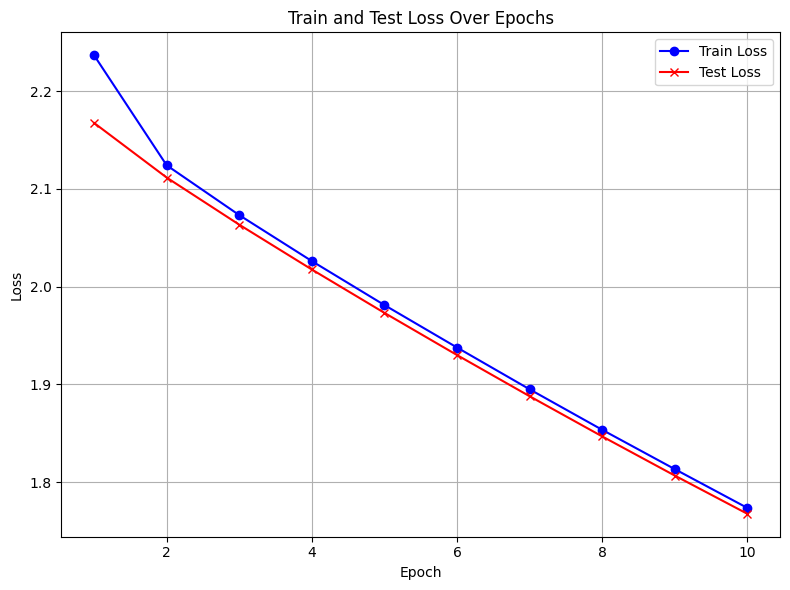
\includegraphics[width=0.5\linewidth]{MLPTrainTestLoss.png}
    \caption{Loss by Epoch for MLP}
    \label{fig:enter-label}
\end{figure}

\begin{figure}[H]
    \centering
    % First figure
    \begin{subfigure}[b]{0.45\linewidth}
        \centering
        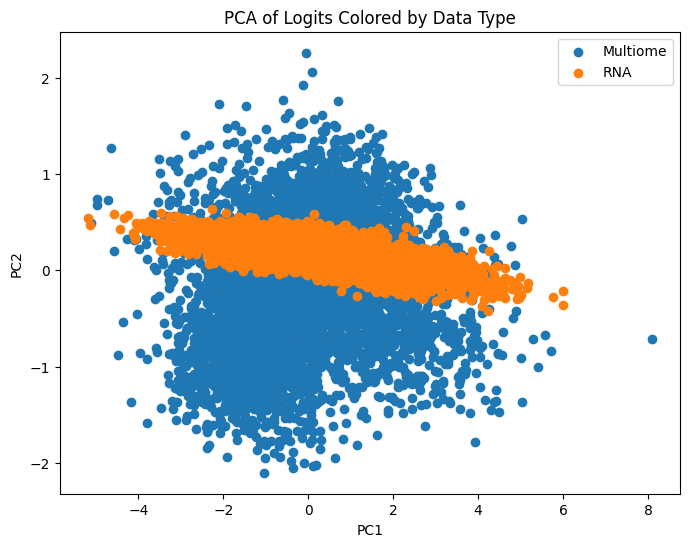
\includegraphics[width=\linewidth]{PCAofTestLogits.png}
        \caption{2D Representation of Logits by Modality for MLP Model}
        \label{fig:figure7}
    \end{subfigure}
    \hfill
    % Second figure
    \begin{subfigure}[b]{0.45\linewidth}
        \centering
        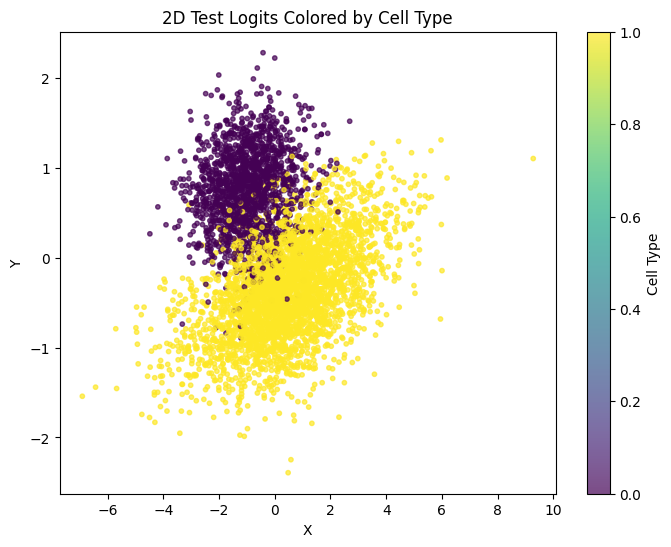
\includegraphics[width=\linewidth]{MLPTestLogitsColoredByCellType.png}
        \caption{2D Representation of Logits by Cell Type for MLP Model}
        \label{fig:figure12}
    \end{subfigure}

    \caption{Comparison of Accuracies by Epoch for MLP}
    \label{fig:comparison}
\end{figure}

\subsection{Multi-Modal Early Fusion Transformer VAE }

The following hyperparameters were used in this model:
 \begin{itemize}
     \item Linear Projection Dimension: 6
     \item Number of Attention Heads: 2
     \item Number of Transformer Encoder Layers: 4
     \item Output Embedding Size: 2
     \item Dropout: 0.3
     \item Number of Parameters in Model: 9,349,070
 \end{itemize}

The train and test loss plots are listed in the figure below.

\begin{figure}[H]
    \centering
    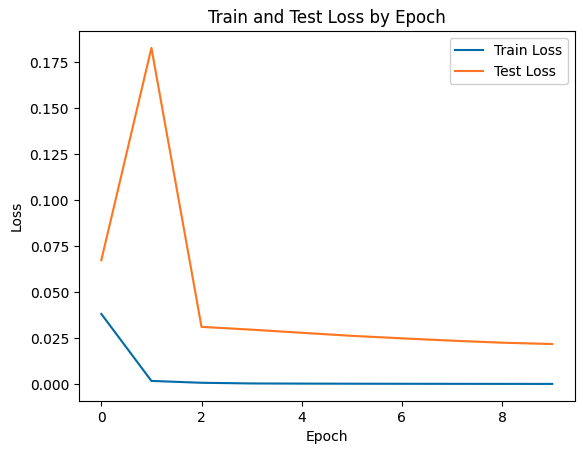
\includegraphics[width=0.5\linewidth]{Figure 3 Rename Final v2.png}
    \caption{Loss by Epoch for Multi-Modal Early Fusion Transformer VAE}
    \label{fig:enter-label}
\end{figure}

\begin{figure}[H]
    \centering
    % First figure
    \begin{subfigure}[b]{0.45\linewidth}
        \centering
        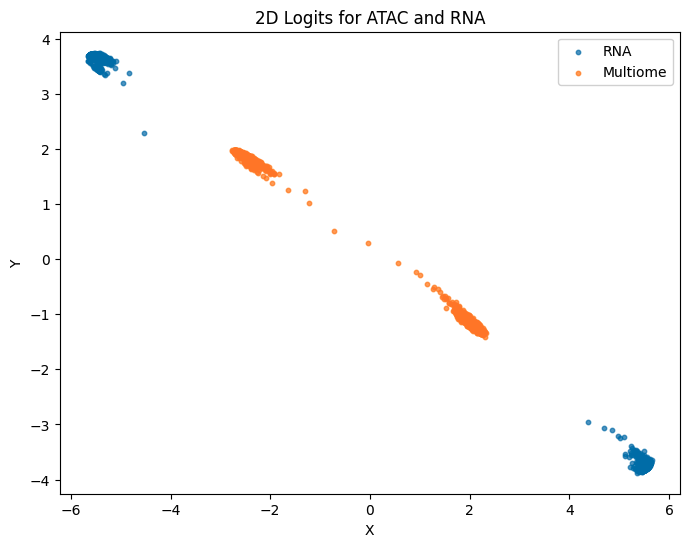
\includegraphics[width=\linewidth]{Figure 4 Final.png}
        \caption{2D Representation of Logits by Modality for VAE}
        \label{fig:figure7}
    \end{subfigure}
    \hfill
    % Second figure
    \begin{subfigure}[b]{0.45\linewidth}
        \centering
        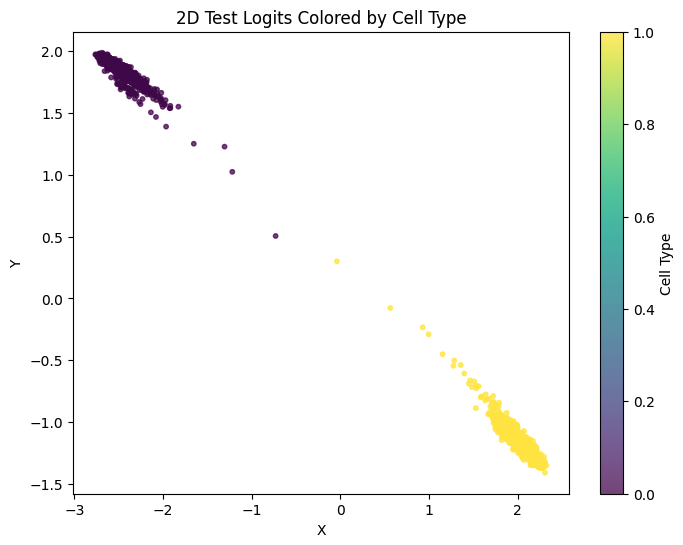
\includegraphics[width=\linewidth]{Figure 5 Final.png}
        \caption{2D Representation of Logits by Cell Type for VAE}
        \label{fig:figure12}
    \end{subfigure}

    \caption{Comparison of Accuracies by Epoch for Multi-Modal Early Fusion Transformer VAE}
    \label{fig:comparison}
\end{figure}

The output embedding plots by cell type and modality are in the figures above.

Our MLP-VAE demonstrates the ability to dimensionally reduce different data modalities. However, without explicitly handling missingness, we find that our embedding produces results similar to the PCA results from the data section.

\subsection{Hyperbolic Multi-Modal Early Fusion Transformer VAE }

The following hyperparameters were used in this model:
 \begin{itemize}
     \item Linear Projection Dimension: 6
     \item Number of Attention Heads: 2
     \item Number of Transformer Encoder Layers: 4
     \item Output Embedding Size: 2
     \item Dropout: 0.3
     \item Number of Parameters in Model: 9,359,162
 \end{itemize}

The hyperbolic model outperforms the baseline model in terms of accuracy. Additionally, it can handle the dataset's feature missingness effectively, while mapping the data into a lower-dimensional space with clear separation between distinct cell types.
\begin{figure}[H]
    \centering
    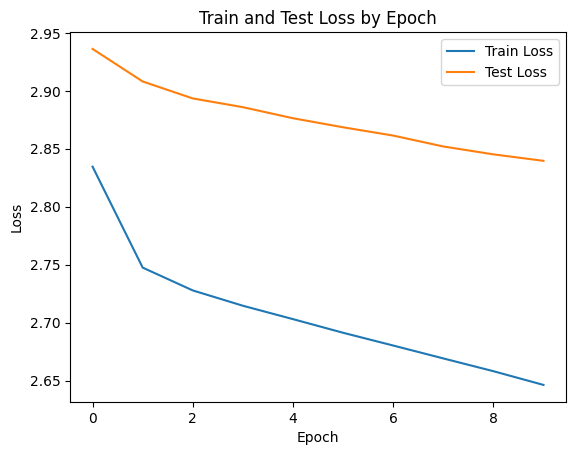
\includegraphics[width=0.5\linewidth]{hyperbolic_loss.png}
    \caption{Loss by Epoch for Hyperbolic Multi-Modal Early Fusion Transformer VAE}
    \label{fig:enter-label}
\end{figure}

\begin{figure}[H]
    \centering
    % First figure
    \begin{subfigure}[b]{0.45\linewidth}
        \centering
        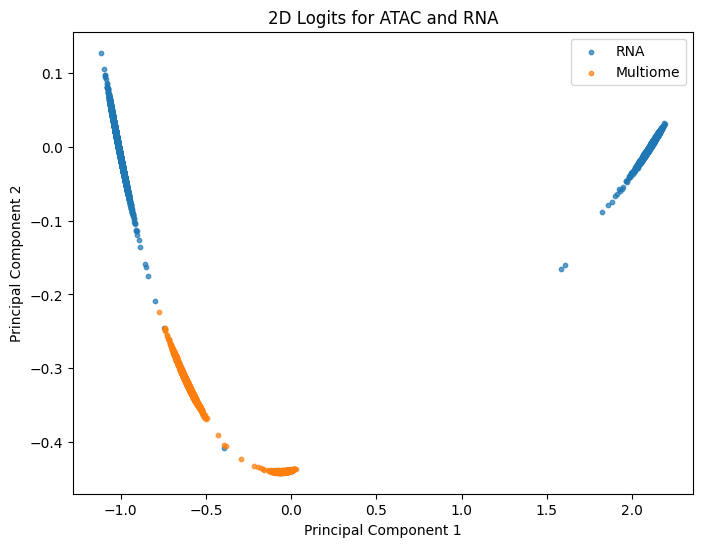
\includegraphics[width=\linewidth]{hyperbolic_train.png}
        \caption{2D Representation of Logits by Modality for Hyperbolic VAE}
        \label{fig:figure7}
    \end{subfigure}
    \hfill
    % Second figure
    \begin{subfigure}[b]{0.45\linewidth}
        \centering
        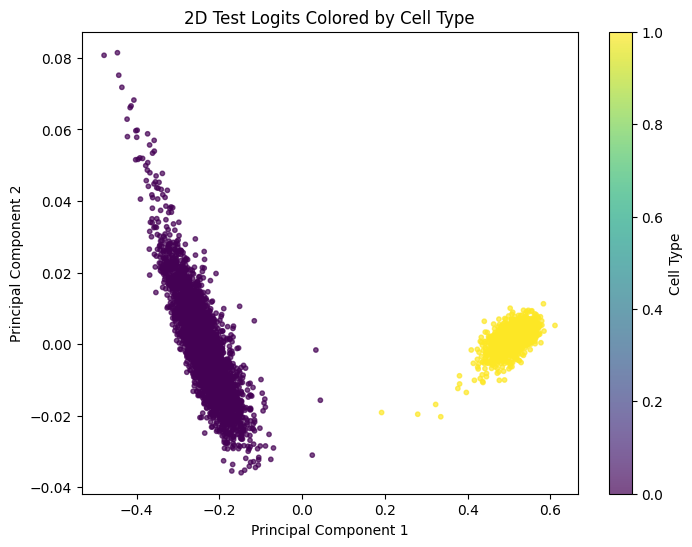
\includegraphics[width=\linewidth]{hyperbolic_test.png}
        \caption{2D Representation of Logits by Cell Type for Hyperbolic Multi-Modal Early Fusion Transformer VAE}
        \label{fig:figure12}
    \end{subfigure}

    \caption{Comparison of Accuracies by Epoch for Hyperbolic Multi-Modal Early Fusion Transformer VAE}
    \label{fig:comparison}
\end{figure}

\section{Discussion}
%Discuss each of the methods MLP-VAE, Hyperbolic VAE, and Transformer, MLP does not handle missingness at all, we need to split our dataset into seperate embeddings in order to handle missingness otherwise we get PCA-like embeddings 

%Initial appraoch was labeling both 0 gene expression and l

% We explored a variety of loss functions during the project including contrastive loss, soft_knn

The transformer had the highest k-NN accuracy at 99\%, followed by MLP at 78\%, and the hyperbolic transformer with 68\%. The Jaccard similarity for all new models were comparable, at values close to 100\%. Additionally, both  training and test datasets had clear separation by modality for the Transformer-based models, highlighting their ability to differentiate between distinct cell types in the reduced-dimensional data.

An important distinction in the Transformer methods was the loss function. Our solution to this at first was to utilize soft K-nearest neighbors to group cells based on cell type, as this was similar to the StabMap paper. Furthermore, we explored using contrastive loss function in our autoencoder models. Ultimately, we found that using Cross Entropy worked the best as it avoided collapsing the output logits into a singular point.

Future work could involve applying our proposed method to additional datasets, to assess its generalization and robustness across different domains. For example, the StabMap paper explores applications across several common datasets that our work could generalize to as well. Additionally, it would be beneficial to explore alternative loss functions that may further optimize the model's performance. Further study could be done in applying contrastive loss functions such as cosine similarity to our model, while treating shared features be Finally, another avenue of investigation is the exploration of different clustering strategies for the modalities, such as evaluating similarity based on gene expression rather than cell type, which could provide new insights into the underlying structure of the data.
\section*{References}
\nocite{*}
\printbibliography[heading=none]

\end{document}
